\section{RESULTS}\label{sec:4experiment}
In this section, we detail the evaluation results for our system.

\subsection{Evaluation of Subcomponents}
We focus on the detection accuracy about five events, that are body posture, the body rollover, the hand position, the micro body movement and the acoustic events.
%, the classification of micro body movement

\subsubsection{Sleep Posture Classification Performance}
\label{subsub:bodyposture}

We test the overall classification performance of different body postures. The groundtruth of body postures are recorded by the cameras. \textcolor{blue}{We use a modified cross-validation approach, which is different from the traditional leave-one-out cross-validation approach. We train the classifier by using only a single user's data, and tested the rest fourteen users.} The motivation for using data from a single user as training data is to highlight the capability of \systemname to accurately characterize body posture with very little training data, while at the same time being able to generalize across users. \textcolor{blue}{Using our method can not only achieve the purpose of cross-validation, that is, the results are more fair and reliable, but also get results in a shorter time, reduce the time cost.} The final performance is then calculated as the averaged accuracy across the 15 folds; as shown in Fig.~\ref{fig:posture_zhu}. We can observe that the posture detection accuracy is consistently high across all users, and does not show major variations across users. This good performance benefits from the distinct characteristics of arm position under different sleeping postures. Compared to results reported for SleepMonitor~\cite{sleepmonitor}, \systemname consistently improves performance which is mainly due to the template-based classifier that we use to verify classifications of the prone and supine states. In particular, \systemname achieves around $5$ percentage units higher performance on the prone state than SleepMonitor and overall has a lower false positive rate.

\begin{figure}
	\centering
	\begin{minipage}{.5\textwidth}
	 \centering
	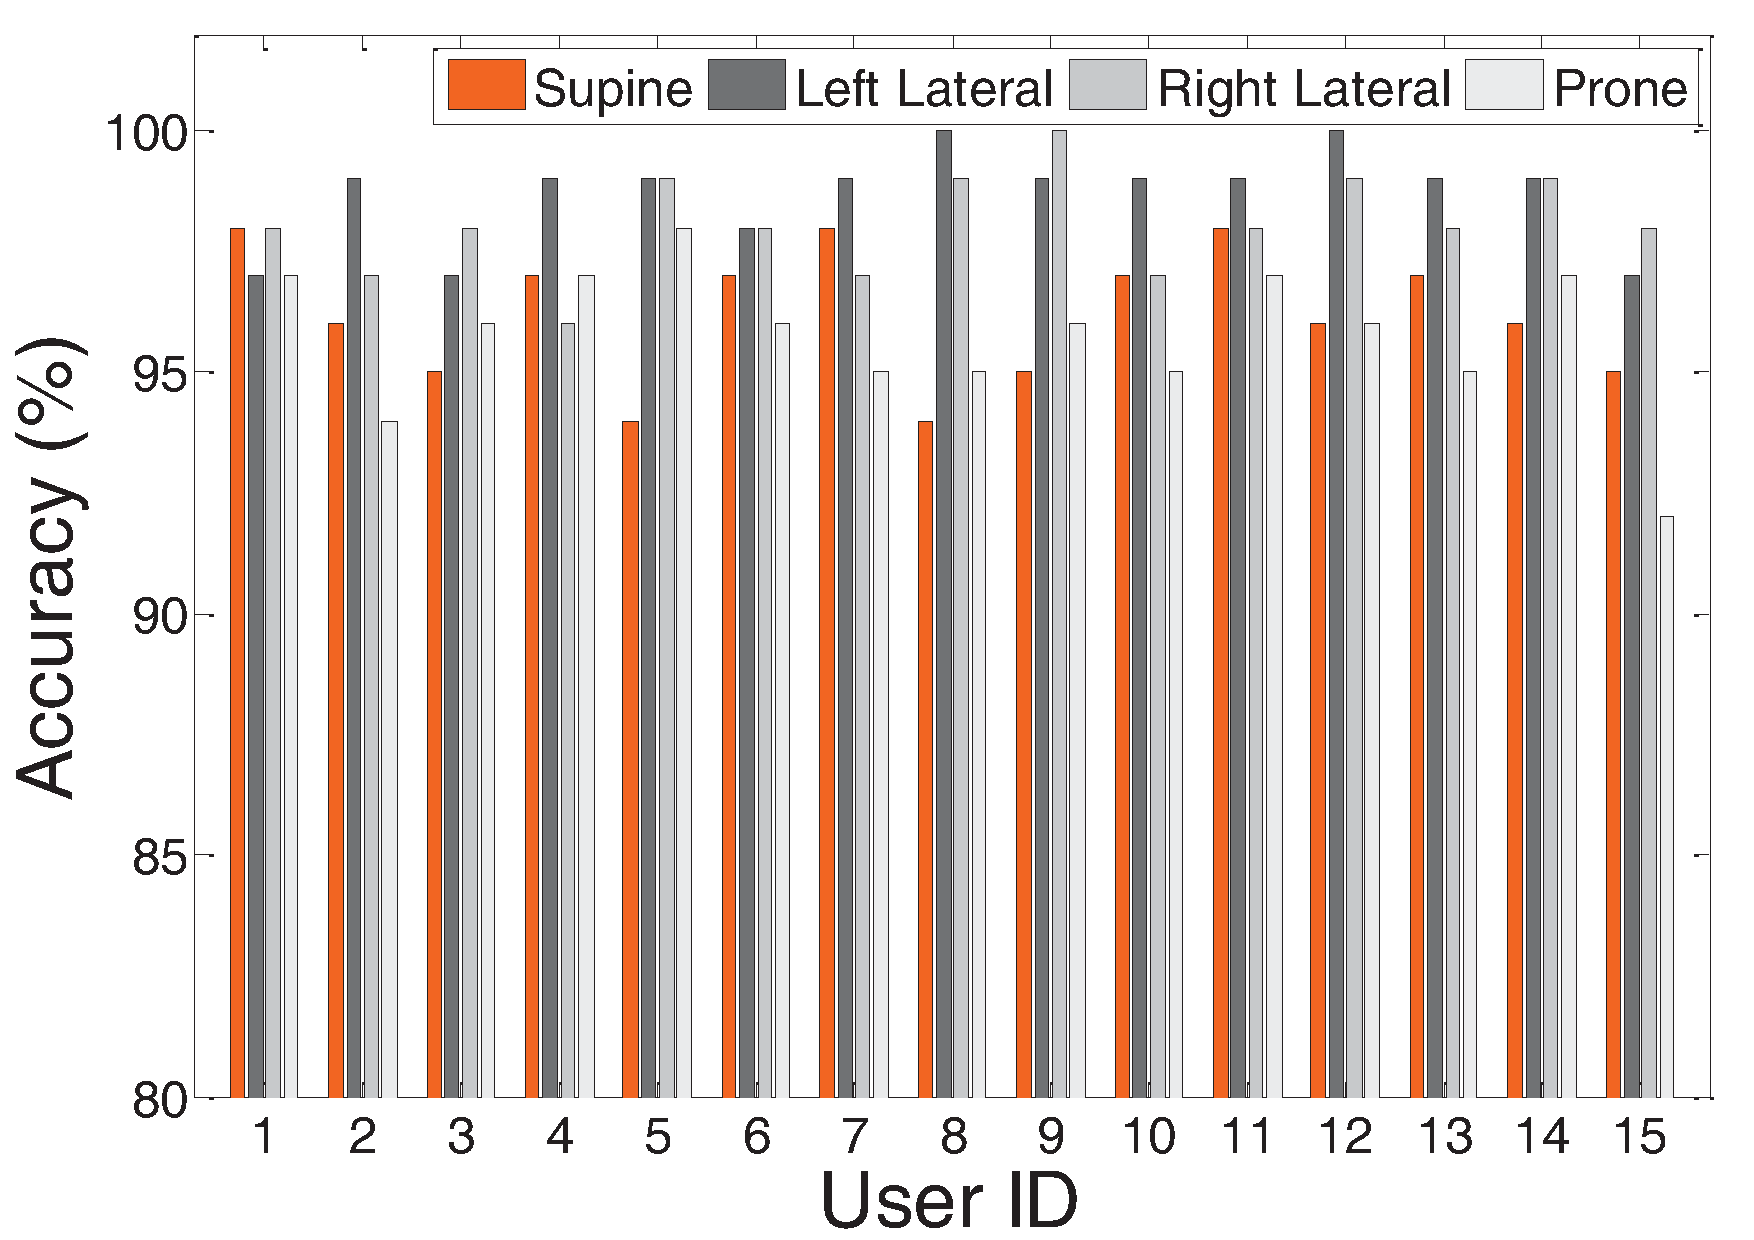
\includegraphics[width=0.95\linewidth]{Figures/posture_zhu.pdf}
	\caption{Detection accuracy of body postures.}\label{fig:posture_zhu}
	\end{minipage}%
	\begin{minipage}{.5\textwidth}
			\centering
		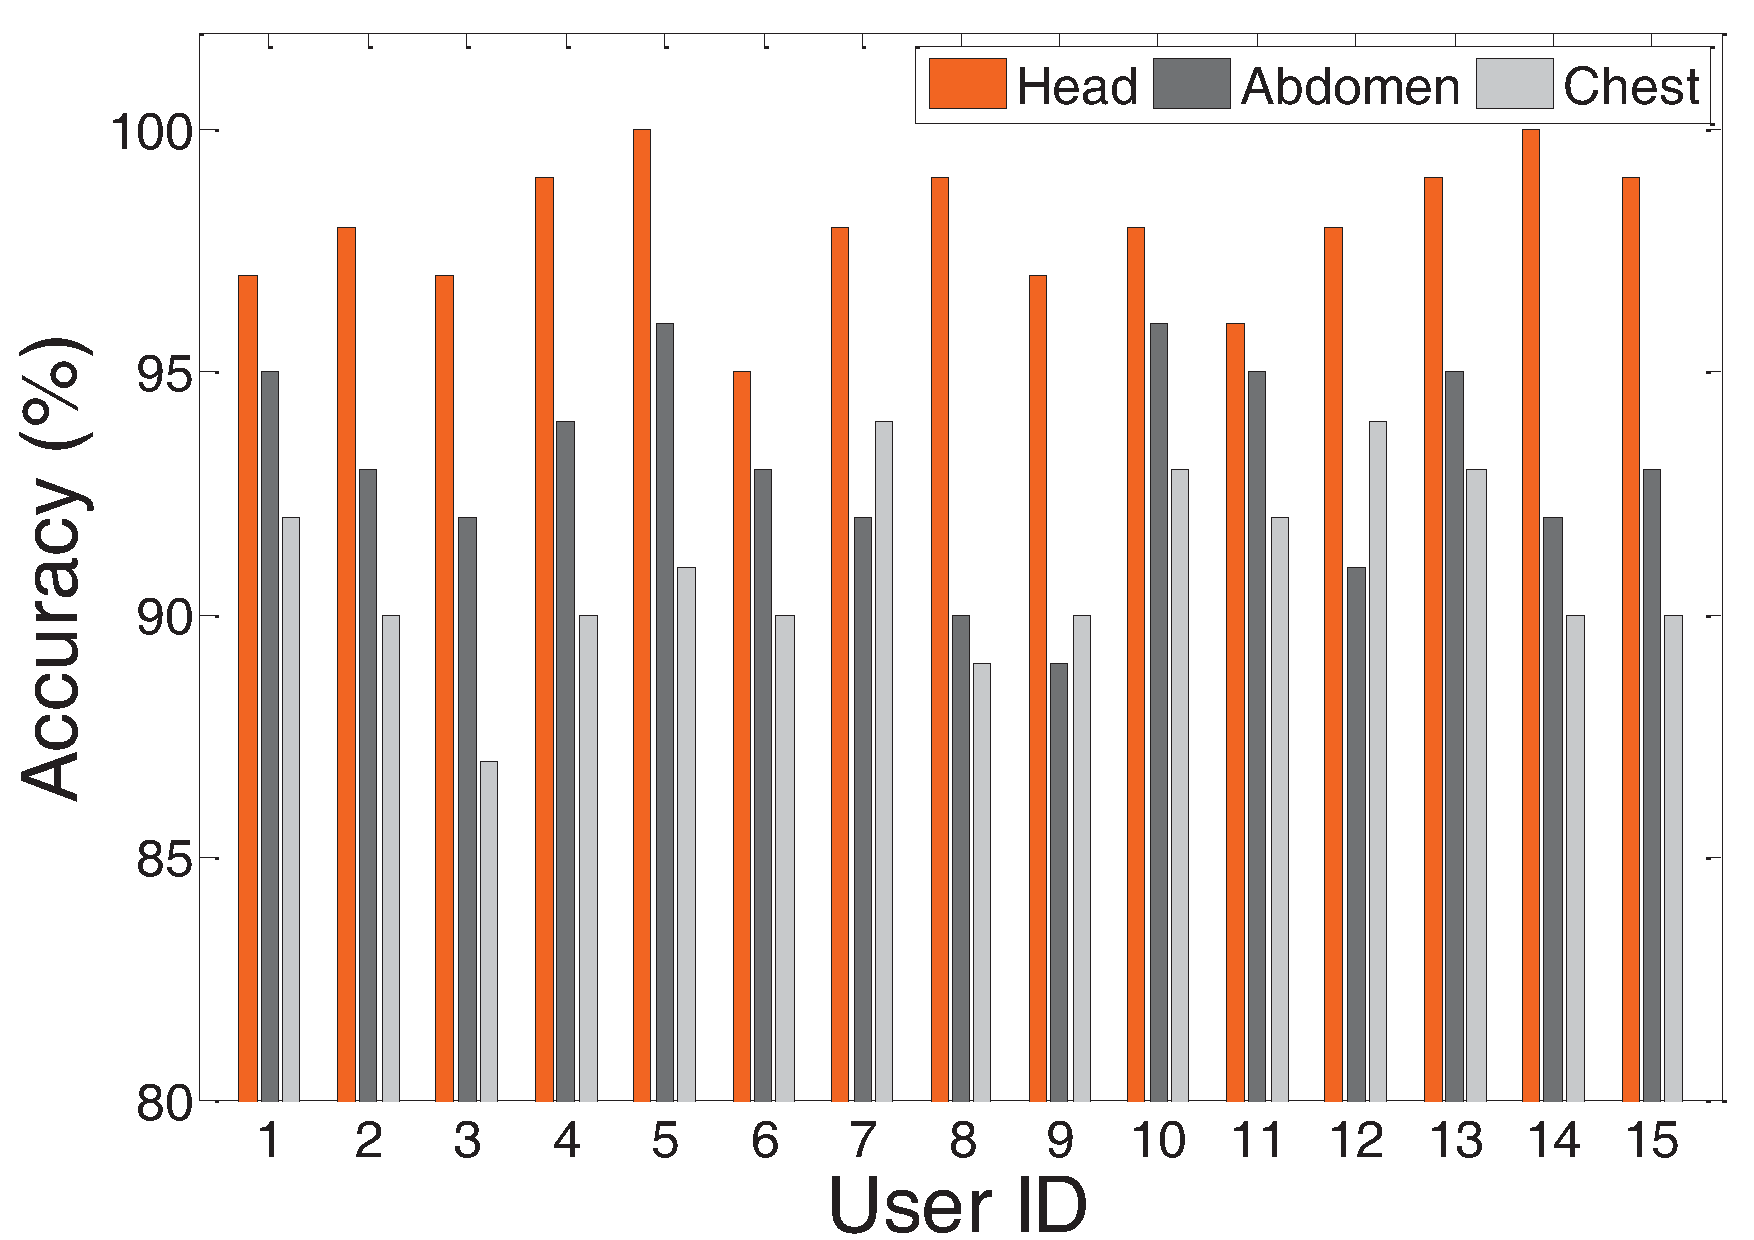
\includegraphics[width=0.95\linewidth]{Figures/handposition_zhu.pdf}
		\caption{Identification accuracy of hand positions.}\label{fig:hand_zhu}
	\end{minipage}
\end{figure}

\begin{table}[!thbp]\footnotesize
%	\tabcolsep1pt
	\centering  % ������
	%\renewcommand\arraystretch{0.277}
	%\caption{The confusion matrix of body posture classification.}\label{tab:posture}
	%\noindent\makebox{%
	%\begin{tabular}{1\textwidth}{ c | c | c | c | c | c | c}
	\renewcommand\arraystretch{0.3}
	\caption{The confusion matrix of body posture classification.}\label{tab:posture}
	\begin{tabular}{c| c | c | c | c | c | c}
		\cline{1-7}
		&\multicolumn{1}{ c|}{ }
		& \multicolumn{4}{ c|}{ }\\
		\multirow{2}*{}
		&\multicolumn{1}{c|}{\multirow{2}*{{Result}}}
		&\multicolumn{4}{c|}{{Prediction}}
		& \multirow{4}*{{Recall}} \\
		%&\multicolumn{5}{ c |}{\textbf{\small Prediction}} \\
		% & \multicolumn{5}{ c |}{ } \\
		\cline{3-6}
		& & & & & \\
		\multicolumn{1}{c|}{{}}
		&  \multicolumn{1}{c|}{{}}
		&  \multicolumn{1}{c|}{{Supine}}
		&  \multicolumn{1}{c|}{{Left Lateral}}
		&  \multicolumn{1}{c|}{{Right Lateral}}
		&  \multicolumn{1}{c|}{{Prone}}   \\
		& & & & & \\
		\cline{1-7}
		& & & & & \\
		\multirow{5}{*}{\begin{sideways}{{Groundtruth}}\end{sideways}}
		&   {Supine}   & {\bf{{1182}}}    &   $25$      &   $4$      &   $9$    &   {96.7\%}\\
		& & & & & \\
		\cline{2-7}
		& & & & & \\
		&   {Left Lateral}   &   $6$      &   {\bf{{1292}}}     &   $0$      &   $0$   &   {99.5\%} \\
		& & & & & \\
		\cline{2-7}
		& & & & & \\
		&   {Right Lateral}   &   $7$      &   $0$      &  {\bf{{1275}}}      &   $12$  &   {98.5\%}  \\
		& & & & & \\
		\cline{2-7}
		& & & & & \\
		&   {Prone}   &   $19$      &   $2$      &   $3$      &   {\bf{{567}}}   &   {95.9\%} \\
		& & & & & \\
		\cline{1-7}
		& & & & & \\
		&   {Precision}    &   {97.3 \%}   &   {98.0\%}   &   {99.5\%}   &   {96.4\%}    \\
		& & & & & \\
		\cline{1-7}
	\end{tabular}
\end{table}

To have a deep evaluation about the sleep posture detection, we randomly choose one user to train the classifier. Then we calculate the detection precision and recall across postures. \textcolor{blue}{The averaged results across our 15 participants is shown in Table \ref{tab:posture}.} The values in blocks are the corresponding numbers of four sleep postures from 14 test users. Due to that the angle features of acceleration are similar between the supine posture with hand putting on the head and the left-lateral posture, a small amount of the supine postures are classified as left lateral.  The total amount of the prone posture is less than the number of other postures. It suggests that most people are not accustomed to sleep in the prone posture, because it is neither healthy nor comfortable. In conclude, Table \ref{tab:posture} shows the outstanding detection performance.



\subsubsection{Performance of body rollover counting}
To verify the efficiency of body rollover detection algorithm, we compare each user's  body rollover number detected by {\systemname} with the groundtruth recorded by camera. The performance is showed in Table \ref{tab:rollver}. We can see that User 3, User 4 and User 13 have an unusually high number. For User 3 and User 4, they have difficulty in falling asleep due to the sleep disorder.  User 13 needs to rollover frequently because of  his loudly snoring. For all the 15 users, the detection accuracies are all very high, and the least one is still 87\%. Thus {\systemname} can accurately distinguish the large hand movement from the body rollover in bed. What's more, detecting errors in body rollover events will not have a significant impact on our end result, because the division of  sleep stages is a comprehensive consideration of all the detected features in each stage, such as micro body movement and acoustic events.

\begin{table}[!thbp]\footnotesize
  %\centering  % ������
 % \tabcolsep 1pt
  %\arrayrulewidth1pt
  \caption{Detection accuracy of body rollover.}\label{tab:rollver}
   \renewcommand\arraystretch{1}{\multirowsetup}{\centering}
        \begin{tabular}{cccccccccccccccc}
        \toprule
         \textbf{User}    & 1& 2  & 3& 4& 5& 6& 7& 8& 9& 10& 11& 12& 13& 14& 15\\
        \midrule
         \rowcolor{Gray}      {\textcolor{blue}{Groundtruth of body rollovers}}  &231&204&442&397&198&101&196&164&193&208&131&205&342&149&156 \\
                 { Accuracy} &91\%& 94\% &88\%&93\%&96\%&94\%&87\%&90\% &93\% &94\% &92\% &94\% &89\% &90\% &95\%\\
        \bottomrule
 \end{tabular}
\end{table}

\subsubsection{Performance of hand position recognition}
To test the recognition performance of different hand positions, {\systemname} uses the cross-validation approach presented in \ref{subsub:bodyposture} with only one user's data at a time to train the classifier and the remaining 14 users' data as the test sets. The classifier for detecting the hand movement trajectory is combined with the detection of periodic signals caused by respiration, then the hand position on the chest (or abdomen or head) can be identified. Fig. \ref{fig:hand_zhu} illustrates the accuracy of hand position across 15 users. As we can see that with just one set of training data, the accuracies for different users are all higher than 87\%. Therefore, our system can achieve a satisfied identification accuracy for different hand positions. Moreover, we find that at least four out of fifteen participants tend to put their hands on their heads; one participate unconsciously puts his hand on his chest which makes him have nightmares. Those are all bad habits disrupting a good sleep.  {\systemname} can report such key findings to improve the users' sleep qualities.


\subsubsection{Performance of micro body movement detection}
To assess the detection accuracy of micro body movement, we manually label the ground truth  recorded by the camera during sleep, including hand moving, arm raising, and body trembling. We also use the accelerometer embedded in the smartphone which placed on the bed to record the occurrence of micro body movements, so as to avoid missing some movements such as trembling concealed by the quilt. \textcolor{blue}{For the acceleration data collected by smartphone, we first smooth the acceleration along the three axes, calculate Root Sum Square (RSS) to merge them, and obtain the first-order derivative of the merged acceleration. And then we use the threshold detection method to mark the occurrence of motion. Since body trembling is the easiest to be covered, we only focus on such events. So we use smartphone to detect the occurrence of events and the classification of the event is not performed.} Fig. \ref{fig:micro_movement_zhu} illustrates the detection accuracy across 15 users. It shows that the accuracies for all users are very close, that is, there will be no major changes between users. And from Fig. \ref{fig:micro_combine}, we find that even though the worst classification result belongs to the hand movement, the average precision value and recall value still exceed 75\%. The averaged accuracies of arm raising and body trembling are 93\% and 84\%, respectively. Because the training data volume for the hand movement and body trembling is small, so the performance can be improved by setting each user a threshold by collecting a longer term's sleeping data. In addition, the purpose of  micro body movement detection is to detect different sleep stages, and the hand movement usually appears in all sleep stages, thus the poor accuracy of hand moving does not have a significant impact on the final result.


\begin{figure}
	\centering
	\begin{minipage}{.5\textwidth}
		 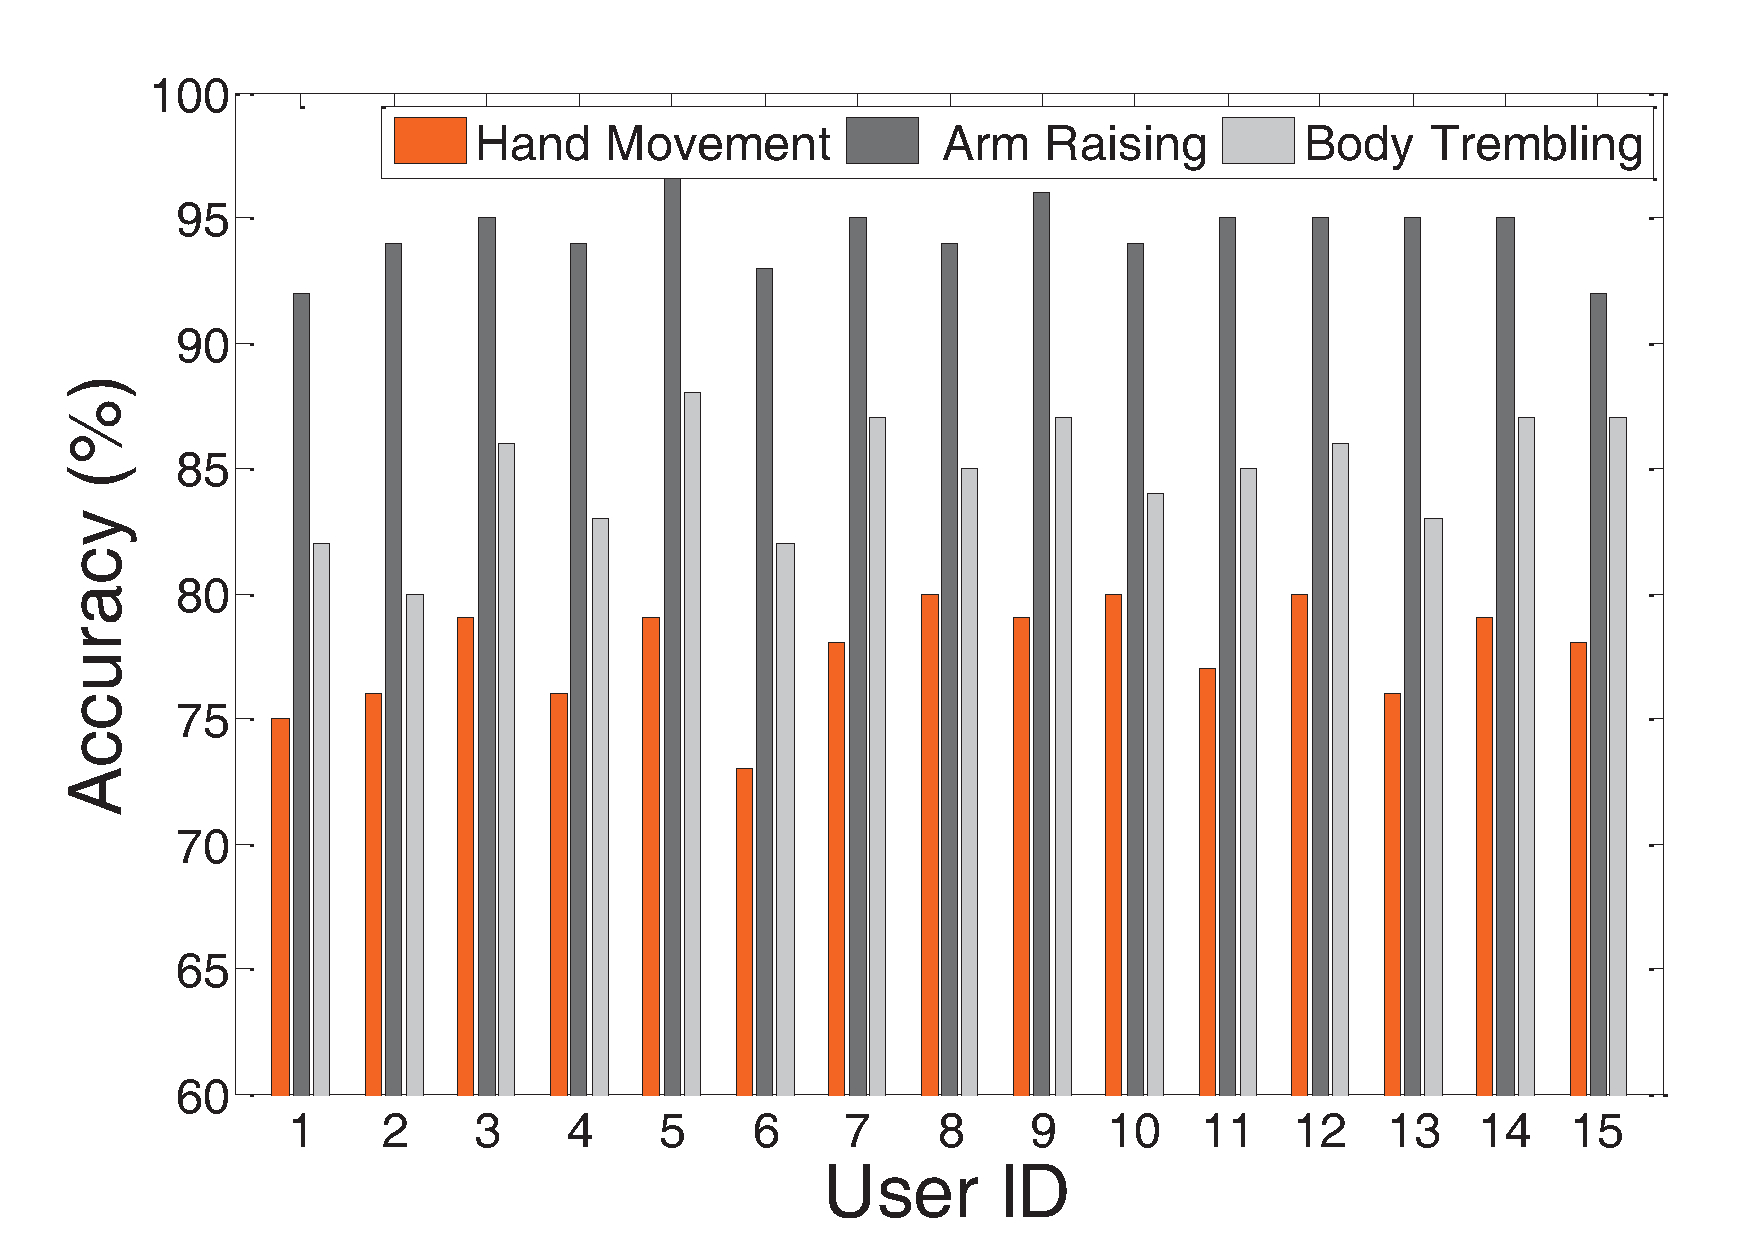
\includegraphics[width=6.5cm,height=4.7cm]{Figures/micro_movement_zhu.pdf}
		\caption{Detection accuracy of micro body movement.}\label{fig:micro_movement_zhu}	
	\end{minipage}%
	\begin{minipage}{.5\textwidth}
	 \centering
	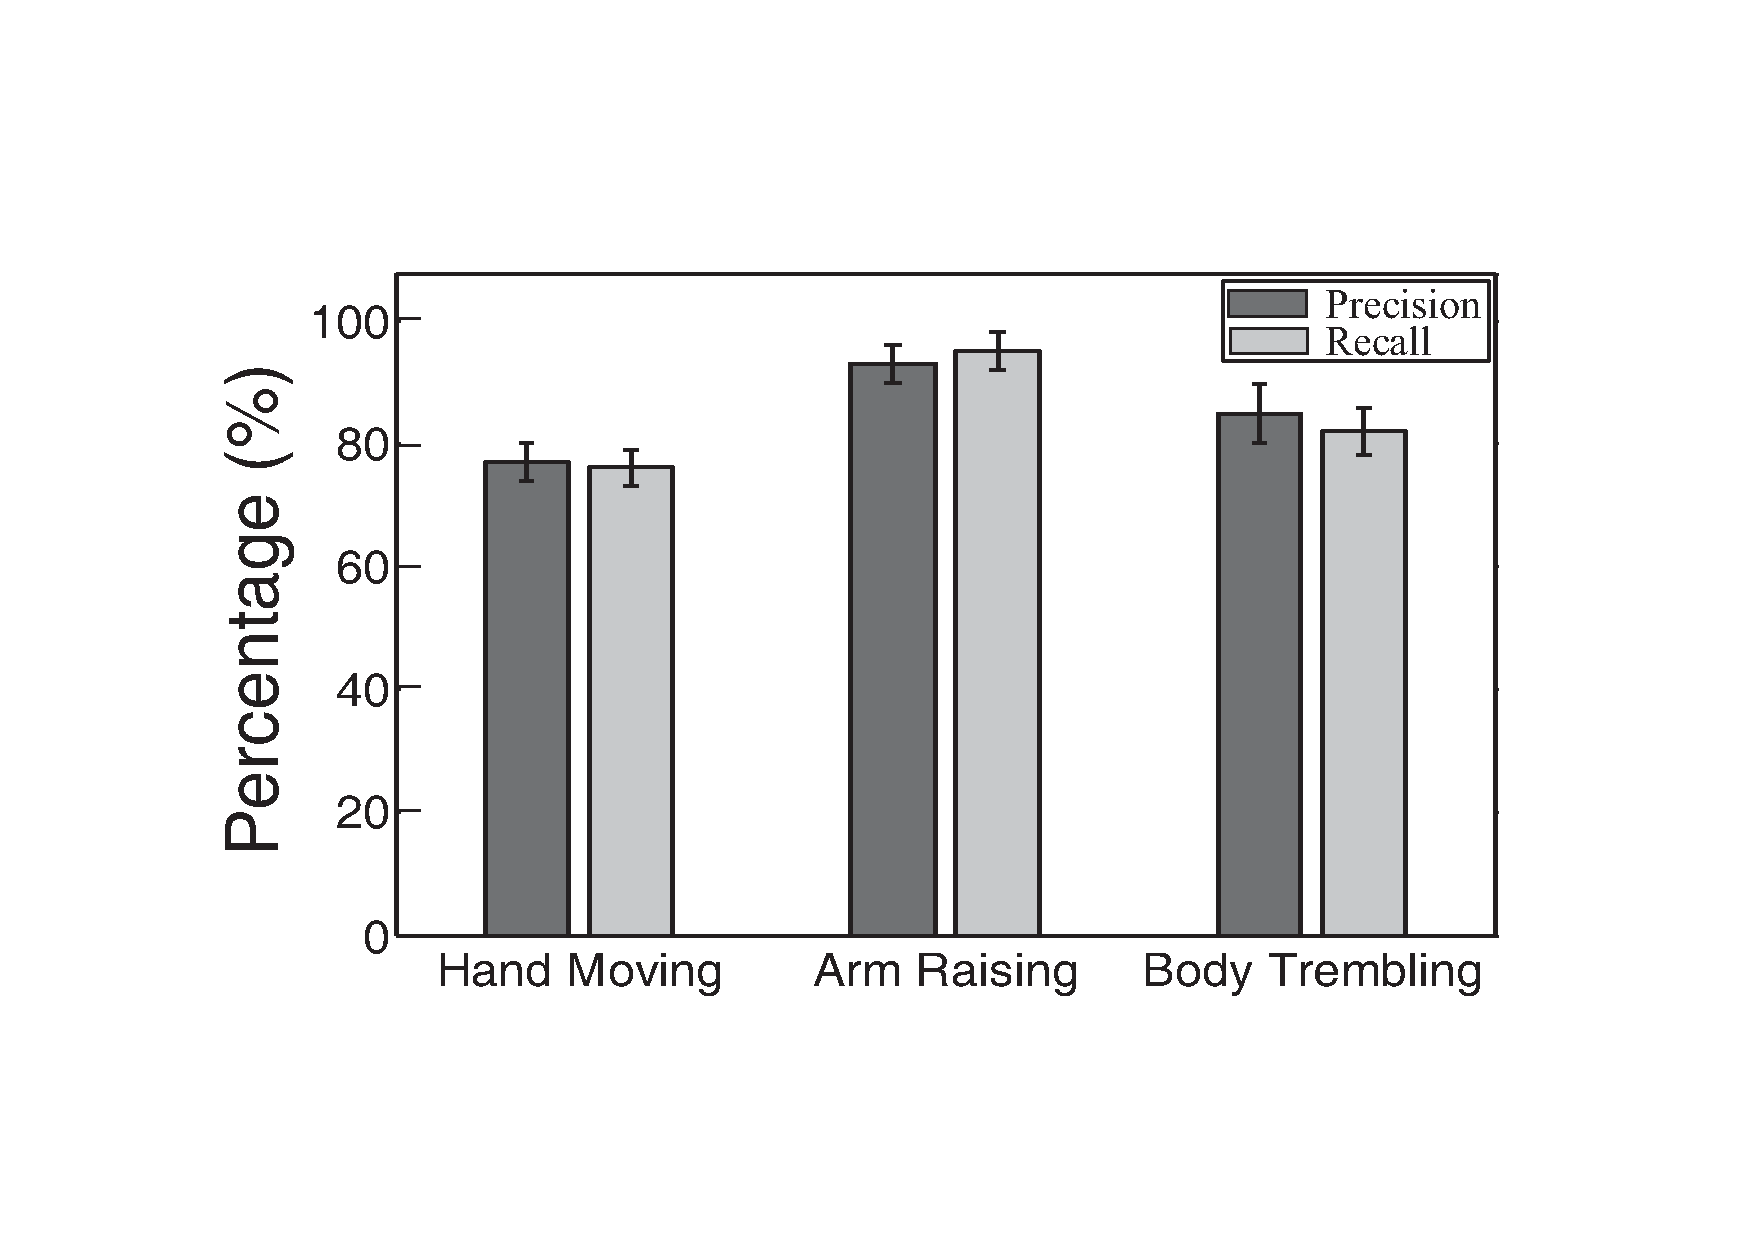
\includegraphics[width=6.5cm,height=4.7cm]{Figures/micro_combine1.pdf}
	\caption{Performance of micro body movement detection.}\label{fig:micro_combine}
	\end{minipage}
\end{figure}



 \subsubsection{Performance of acoustic events detection}
To study the detection accuracies of different acoustic events, we compare the ground truth recorded by the camera with the detected results by our system. Table \ref{tab:sound} shows the results across 15 participants. We can see that the precision for cough event is 88.9\% and a little than other three events. The reason is that different user's cough patterns are different, the pre-defined parameters in the detection model does not include all possible patterns. \textcolor{blue}{For example, some people have a fast and continuous pattern of coughing, while others have a slower intermittent pattern.} In fact, we train these parameters, namely the "interval", "duration" and "frequency" of acoustic events, with only 120 sets of nighttime sound data. Those data come from 40 (21 males and 19 females) volunteers of different ages (from 15 to 60 years old) who are prone to snoring, coughing, or somniloquy at night. To further improve the detection accuracy, we can train particular parameters for different users. \textcolor{blue}{And we can further expand the training data to include more possible patterns, and can also make reasonable estimates of the possible patterns to refine the range of parameters and thus increase the accuracy.}


\begin{table}[!thbp]\footnotesize
% \tabcolsep1pt
  \centering  % ������
 \renewcommand\arraystretch{0.3}
  \caption{The confusion matrix of acoustic events detection.}\label{tab:sound}
\begin{tabular}{c| c | c | c | c | c | c}
   \hline
   &\multicolumn{1}{ c|}{ }
   & \multicolumn{4}{ c|}{ }\\
   \multirow{2}*{}
&\multicolumn{1}{c|}{\multirow{2}*{{ Result}}}
&\multicolumn{4}{c|}{{ Prediction}}
& \multirow{4}*{{ Recall}} \\
    %&\multicolumn{5}{ c |}{\textbf{\small Prediction}} \\
   % & \multicolumn{5}{ c |}{ } \\
    \cline{3-6}
    & & & & & \\
    \multicolumn{1}{c|}{{}}
    &  \multicolumn{1}{c|}{{}}
    &  \multicolumn{1}{c|}{{ Snore}}
    &  \multicolumn{1}{c|}{{ Cough}}
    &  \multicolumn{1}{c|}{{ Somniloquy}}
    &  \multicolumn{1}{c|}{{ Other}}   \\
    & & & & & \\
     \cline{1-7}
    & & & & & \\
    \multirow{5}{*}{\begin{sideways}{{ Groundtruth}}\end{sideways}}
    &   { Snore}   & {\bf{{96}}}    &   $0$      &   $0$      &   $9$    &   {91.4\%}\\
    & & & & & \\
    \cline{2-7}
    & & & & & \\
   &   { Cough}   &   $3$      &   {\bf{{64}}}     &   $0$      &   $4$   &   {90.1\%} \\
    & & & & & \\
     \cline{2-7}
    & & & & & \\
    &   { Somniloquy}   &   $0$      &   $3$      &  {\bf{{42}}}      &   $2$  &   {89.4\%}  \\
    & & & & & \\
     \cline{2-7}
    & & & & & \\
    &   { Other}   &   $0$      &   $5$      &   $4$      &   {\bf{{325}}}   &   {97.3\%} \\
    & & & & & \\
    \hline
    & & & & & \\
    &   { Precision}      &   {96.9\%}   &   {88.9\%}   &   {91.3\%}   &   {95.6\%}    \\
    & & & & & \\
    \hline
   \end{tabular}
\end{table}


\subsection{Overall performance \label{sec:overall_per}}

\subsubsection{Performance of sleep stage detection}

In order to prove that the detected events not only reflect the user's sleep habits, but also effectively identify the sleep stages to assess the sleep quality, we regard the reported results from Fitbit Charge2 as the ground truth. There are 50 sets of nocturnal sleep data selected from 210 sets of sleep data, \textcolor{blue}{in order to effectively assess performance while also reducing the time cost of the assessment. And to make the selection fairly and avoid overfitting,} we randomly pick at least 3 sets of data for each participant. For reflecting the sleep stage change carefully, \textcolor{blue}{{\systemname} use event-driven detection. When there is no sleep event detected in 15 minutes, we evaluates the sleep stage. When an event occurs, we immediately evaluates the sleep stage and use this time as the starting point for the next 15 minutes.} The averaged precision value and recall value are shown in Table \ref{tab:sleep stage}. It indicates that though {\systemname} may make misjudgement between the light sleep and REM, the overall performance is satisfying.

\begin{table}[!thbp]\footnotesize
%	\tabcolsep1pt
	\centering  % ������
	\renewcommand\arraystretch{0.4}
	\caption{{The confusion matrix of sleep stage detection.}}\label{tab:sleep stage}
	\begin{tabular}{c| c | c | c | c | c}
		\hline
		&\multicolumn{1}{ c|}{ }
		& \multicolumn{3}{ c|}{ }\\
		\multirow{2}*{}
		&\multicolumn{1}{c|}{\multirow{2}*{{ Result}}}
		&\multicolumn{3}{c|}{{ Prediction}}
		& \multirow{3}*{{ Recall}} \\
		%&\multicolumn{5}{ c |}{\textbf{\small Prediction}} \\
		% & \multicolumn{5}{ c |}{ } \\
		\cline{3-5}
		& & & & & \\
		\multicolumn{1}{c|}{{}}
		&  \multicolumn{1}{c|}{{}}
		&  \multicolumn{1}{c|}{{ REM}}
		&  \multicolumn{1}{c|}{{ Light Sleep}}
		&  \multicolumn{1}{c|}{{ Deep Sleep}} \\
	%	& & & & & \\
		\cline{1-6}
		& & & & & \\
		\multirow{1}{*}{\begin{sideways}{{ Groundtruth}}\end{sideways}}
		&   { REM}   & {\bf{{476}}}    &   $143$      &   $61$     &   {70.0\%}\\
		& & & & & \\
		\cline{2-6}
		& & & & & \\
		&   { Light Sleep}   &   $131$      &   {\bf{{508}}}     &   $91$      &   {69.6\%} \\
		& & & & & \\
		\cline{2-6}
		& & & & & \\
		&   { Deep Sleep}   &   $63$      &   $113$      &  {\bf{{262}}}      &   {59.8\%}  \\
		& & & & & \\
		\cline{1-6}
		& & & & & \\
		&   { Precision}      &   {71.0\%}   &   {66.5\%}   &   {63.3\%}   \\
		& & & & & \\
		\hline
	\end{tabular}
\end{table}

\subsubsection{Effect of respiratory amplitude on sleep stage detection}
When we detect different sleep stages, we also consider the respiratory amplitude when the hand's position is in the abdomen or chest. To assess the effectiveness of respiration amplitude estimation, we evaluate the performance of the sleep stage detection in two cases, that are with and without taking the respiration amplitude into account. The performance of sleep stage detection is shown in Table \ref{tab:respiratory}. For three different sleep stages, both the precision and recall values are improved with the help of respiration amplitude estimation. \textcolor{blue}{In fact, respiratory frequency can also be used as a feature to help us to detect sleep stages. But in fact  their essence the same. The difference in respiratory amplitude will also affect the difference in respiratory frequency, because when the respiratory amplitude is large, the time taken for one breath will be long, and the frequency of breathing will be slower. In {\systemname}, we choose the respiratory amplitude because the feature is very intuitive.}

\begin{table}[!thbp]\footnotesize
	\centering  % ������
	\renewcommand\arraystretch{0.3}
	\caption{Effect of respiration amplitude estimation.}\label{tab:respiratory}
	\begin{tabular}{c| c | c | c | c | c | c| c |}
		\cline{2-8}
		&\multicolumn{1}{ c|}{ }
		&\multicolumn{2}{ c|}{ }
		&\multicolumn{2}{ c|}{ }
		& \multicolumn{2}{ c|}{ }\\
		%  \multirow{4}*{}
		&\multicolumn{1}{c|}{}
		&\multicolumn{2}{c|}{\textbf{\footnotesize REM}}
		&\multicolumn{2}{c|}{\textbf{\footnotesize Light Sleep}}
		&\multicolumn{2}{c|}{\textbf{\footnotesize Deep Sleep}} \\
		%&\multicolumn{5}{ c |}{\textbf{\small Prediction}} \\
		% & \multicolumn{5}{ c |}{ } \\
		\cline{2-8}
		& & & & & & &\\
		\multicolumn{1}{c|}{\textbf{}}
		&  \multicolumn{1}{c|}{\textbf{Features}}
		&  \multicolumn{1}{c|}{\footnotesize Precision}
		&  \multicolumn{1}{c|}{\footnotesize Recall}
		&  \multicolumn{1}{c|}{\footnotesize Precision}
		&  \multicolumn{1}{c|}{\footnotesize Recall}
		&  \multicolumn{1}{c|}{\footnotesize Precision}
		&  \multicolumn{1}{c|}{\footnotesize Recall}\\
		& & & & & & &\\
		\cline{2-8}
		& & & & & & &\\
		\multirow{5}{*}
		&   \textbf{\footnotesize Without Respiration Amplitude}   & $62.9\%$    &   $63.4\%$      &   $59.4\%$      &   $63.9\%$    &   $57.7\%$ &  $54.1\%$ \\
		& & & & & & &\\
		\cline{2-8}
		& & & & & & &\\
		&   \textbf{\footnotesize With Respiration Amplitude}   &   $71.0\%$      &   $70.0\%$     &   $66.5\%$      &   $69.7\%$   &   $63.3\%$ &   $59.8\%$ \\
		& & & & & & &\\
		
		\cline{2-8}
		
	\end{tabular}
\end{table}

\subsubsection{Performance comparison}
We compare {\systemname} with two state-of-the-art work, the sleep detection app Sleep As Android and smartphone-based system Sleep Hunter \cite{gu2016sleep}.  Considering that Sleep As Android can only detect light sleep stage and deep sleep stage, we only compare the performance of these two stages. Table \ref{tab:comparison} shows the detection results.
As we can see, {\systemname}  performs much better than Sleep As Android and slightly better than Sleep Hunter. This good performance comes from the incorporation of rich and complicated sleep events. Therefore, our system helps users understand their sleep more easily and improve  sleep quality more effectively.

  \begin{table}[!thbp]\footnotesize
 	\centering  % ������
 	\renewcommand\arraystretch{0.3}
 	\caption{Performance of sleep stage detection comparison.}\label{tab:comparison}
 	\begin{tabular}{c| c | c | c | c | c |}
 		\cline{2-6}
 		&\multicolumn{1}{ c|}{ }
 		&\multicolumn{2}{ c|}{ }
 		&\multicolumn{2}{ c|}{ }\\
 		%  \multirow{4}*{}
 		&\multicolumn{1}{c|}{}
 		&\multicolumn{2}{c|}{\textbf{\footnotesize Light Sleep}}
 		&\multicolumn{2}{c|}{\textbf{\footnotesize Deep Sleep}} \\
 		%&\multicolumn{5}{ c |}{\textbf{\small Prediction}} \\
 		% & \multicolumn{5}{ c |}{ } \\
 		\cline{2-6}
 		\multicolumn{1}{c|}{\textbf{}}
 		&  \multicolumn{1}{c|}{\diagbox{System}{Stage}}
 		&  \multicolumn{1}{c|}{\footnotesize Precision}
 		&  \multicolumn{1}{c|}{\footnotesize Recall}
 		&  \multicolumn{1}{c|}{\footnotesize Precision}
 		&  \multicolumn{1}{c|}{\footnotesize Recall}\\
 		\cline{2-6}
 		& & & & & \\
 	%	\multirow{3}{*}
 		&   \textbf{\footnotesize SleepGuard}   & $66.5\%$    &   $69.6\%$      &   $63.3\%$      &   $59.8\%$  \\
 		& & & & &  \\
 		\cline{2-6}
 		& & & & & \\
 		&   \textbf{\footnotesize Sleep As Android}   &   $27.8\%$      &   $35.4\%$     &   $35.7\%$      &   $50.2\%$   \\
 		& & & & &  \\
 		\cline{2-6}
 		& & & & & \\
 		&   \textbf{\footnotesize Sleep Hunter}   &   $66.74\%$      &   $66.11\%$     &   $60.00\%$      &   $50.73\%$   \\
 		& & & & &  \\
 		
 		\cline{2-6}
 		
 	\end{tabular}
 \end{table}


Further, we compare {\systemname}'s functions with 8 other sleep detection products  in Table \ref{tab:function}, including Sleep As Android, Sleep Hunter, sleepMonitor \cite{sleepmonitor}, Sleeptracker \cite{sleeptracker}, Fitbit, isleep \cite{hao2013isleep}, Jawbone \cite{Jawbone} and ubiSleep \cite{pombo2016ubisleep}.  {\systemname} detects a wider range of sleep events and thus provides a better user experience.

\begin{table*}[!thbp]\footnotesize
%\setlength{\abovecaptionskip}{0.8pt}
  \centering  % ������
  \tabcolsep7pt
  %\arrayrulewidth1pt
  \caption{Functions comparision between different systems.}\label{tab:function}
  \renewcommand{\multirowsetup}{\centering}
  \noindent\makebox[\textwidth]{%
        \begin{tabularx}{1.0\textwidth}{|c|c|c|c|c|c|c|}
        \cline{1-7}
        \multicolumn{1}{|c|}{\multirow{2}*{\textbf{\footnotesize System}}}
        &\multicolumn{6}{c|}{\textbf{ \footnotesize Detected Events}} \\
         \cline{2-7}
    &  \multicolumn{1}{c|}{\textbf{ \footnotesize Heart Rate }}
    &  \multicolumn{1}{c|}{\textbf{ \footnotesize Acoustic Event }}
    &  \multicolumn{1}{c|}{\textbf{ \footnotesize Sleep Posture }}
     &  \multicolumn{1}{c|}{\textbf{ \footnotesize Body Movement }}
      &  \multicolumn{1}{c|}{\textbf{ \footnotesize Hand Position}}
       &  \multicolumn{1}{c|}{\textbf{ \footnotesize Sleep Stage}} \\
        \cline{1-7}
        \multirow{7}{2.14cm}
        {\textbf{SleepGuard\\Sleep as Android\\Sleep Hunter\\SleepMonitor\\Sleeptracker\\isleep \\Fitbit\\Jawbone\\ ubiSleep } }
        & &$\checkmark$ & $\checkmark$ &  $\checkmark$  &$\checkmark$ &$\checkmark$\\
        & &$\checkmark$ & & & &$\checkmark$\\
        & & $\checkmark$& &$\checkmark$ & &$\checkmark$\\
        & & & $\checkmark$ & & &\\
        &$\checkmark$ & & & & &$\checkmark$\\
         & &$\checkmark$ &   &$\checkmark$ & &\\
         &$\checkmark$ & & & & &$\checkmark$ \\
        & & & & & &$\checkmark$ \\
        & $\checkmark$&$\checkmark$ & & & &\\
        \cline{1-7}
 \end{tabularx}}
\end{table*}

\subsubsection{User survey \label{sec:user_survey}}
\textcolor{blue}{In order to understand and verify whether the events detected by SLEEPGUARD are really interested or needed by users, we investigated and researched users. The user survey we conducted consisted of two types of people. One is the 15 volunteers who participated in our experiment, we not only conducted a sleep quality assessment for them but also investigated these users�� experience for SLEEPGUARD. And the others do not use our system, so, they only be asked if they were interested in or recognized the events we detected. Therefore, the results of the user survey are also composed of two parts. They are the assessment of sleep quality and the survey of user experience.For the assessment of sleep quality, we asked participants to fill out our questionnaire based on PSQI [16] every morning during the experiments, and compare the results of SLEEPGUARD and Fitbit
measurements with it. The questions in our survey include:}
\begin{enumerate}
  \item Subjective sleep quality (5 levels, 1 for excellent and 5 for worst),
  \item Sleep duration,
  \item Sleep disturbances,
  \item Daytime dysfunction.
\end{enumerate}
For the above four items, each one is rated on a 1 to 5 scale. These scores are first summed to yield a total score, which ranges from 0 to 20. Then we merge every five neighboring scores into one scale and eventually divide the total scores into four levels, recorded as 0, 1, 2 and 3, representing poor, general, good and excellent, respectively. The final sleep quality score comes from the comprehensive scores of above four questionnaires.

\textcolor{blue}{The 14-days averagesleep quality scores from 15 participates are presented in Table \ref{tab:quality}. We also list the sleep quality results obtained from SLEEPGUARD and Fitbit. In Table \ref{tab:quality}, as we can see, these value are the 14-day average results obtained by combining the sleep quality scores for each participant per day. The scores are divided into four levels, recorded as 0, 1, 2 and 3, representing poor, general, good and excellent, respectively. We compared sleep quality scores from {\systemname}, Fitbit, and user surveys. We can see that although {\systemname}'s assessment of sleep quality scores is only consistent with 9 users' subjective feelings. and only slightly better than Fitbit's results.However, results of the {\systemname} assessment are similar to those of the user survey. Possible inconsistencies are scores 2 and 3, that is, good and excellent, score 0 and 1, that is, poor and general, and there are few cases in which bad sleep has been assessed as good. These similar results are acceptable. We also found that when the results of the {\systemname} were inconsistent with the results of the user survey, it was consistent with the Fitbit results. The reason for such a situation may be that, for example, the user feels good about his own sleep but actually still has some neglected problems during sleep, which is detected by the sleep detection device, which is very helpful to the user. So we can find through the user survey these sleep behaviour we detected are indeed effective and beneficial for people, especially for users with sleep problems.}

\textcolor{blue}{In addition, we summarized the sleep problems and habit of the 15 volunteers who participated in our system assessment through a questionnaire survey and quality of sleep assessment. Then we found that there is a participant reported that his arm was always paralyzed, and five participants had poor sleep quality. We can find that the reason why the user's arm is numb is his incorrect sleep habits. The results from {\systemname} showed that he always tends to put his hands on his head, and long-term postures like this will inevitably lead to numbness of the arms. For similar situations, we will inform and remind users of their inappropriate postures and habits, and recommend that users should take measures to improve such situations. And for the poor quality of sleep of users, we analyzed the cause one by one based on events detected by {\systemname}. Through {\systemname}'s detecting, one user showed obvious symptoms of the difficulty of falling asleep and an unusually high number of body rollover. Our further analysis revealed that there was excessive light intensity and frequent noise in his sleeping environment. This may have led to the appearance of these symptoms and thus the poor quality of sleep. Then {\systemname} will recommend that users should focus on and improve his sleeping environment. In fact, this situation is very common that some users often choose to sleeping with a bright light because of one's fear of going to sleep alone. Even if they can also feel that this has an impact on their sleep. But in fact doing so for a long time is very bad for sleep and health. So {\systemname} also gives some suggestions for resolution, for example, do some proper exercise before going to bed or go to sleep with soft music that can be automatically turned off. And there is a user reported that he always had a nightmare at night, which led to poor sleep quality. We analyse the results of {\systemname} and found that user has been accustomed to sleep in the left side, and sometimes the hand is habitually placed on the chest. As \cite{nightmare} points that people who sleep on their left side are more at risk of nightmares. And the oppression of the chest by the hand causes the brain to have an ill hallucination, making it extremely easy to make a nightmare. So {\systemname} suggest to the user based on these two possible reasons, and hope that the user can take some special measures to change it, and recommend that the user can take some additional methods, such as listening to some soothing music to relax before sleep. Another user was detected by {\systemname} to be bothered by long-term snoring, as he himself mentioned. We know that the occurrence of snoring is most likely due to improper sleeping posture, and we also detected that the user is accustomed to sleep in a supine position, so on the one hand, {\systemname} suggests that the user try the sleeping position in the side position. On the other hand, if the situation still does not improve very well, it is recommended that the user go to the hospital in time for a corresponding check to avoid snoring caused by certain diseases. In addition, if we detect that some users are accustomed to sleeping in a prone position, we will remind and advise them because the prone position is bad for health.}

\textcolor{blue}{According to different possible reasons, {\systemname} proposes different reminders and suggestions to users, such as adjusting their sleeping posture, improving the sleeping environment, and consciously avoiding bad sleeping habits. As for how to adjust and avoid them, users can take special, mandatory or medical methods according to their own situation. For example, \cite{posture} present an anti-supine device mimicking the so-called "tennis ball technique" to control sleep posture, in order to improve OSA hypopnoea syndrome. And it is recommended that long-term snoring users perform physical examination so that they can timely The discovery of physical diseases that is most likely to cause snoring such as high blood pressure, cardiovascular and cerebrovascular diseases. In addition, we asked the 15 participants to make appropriate adjustments according to our recommendations and to conduct a return visit survey three weeks later. It was found that some of the users had some symptoms relieved and the average quality of sleep was improved.}
	
\textcolor{blue}{As for the user experience, we can find that most people are praised and interested in these events detected by {\systemname}.} 80\% of participants believe that the detection of sleep posture is very necessary, showing their sleep posture can not only help people to avoid health problems caused by long-term improper sleeping posture, but also help us find out the reasons for the next day's physical discomfort, such as dizziness, muscle soreness may be due to improper sleeping posture. \textcolor{blue}{And there are some users are troubled by snoring. This may be due to improper sleeping posture. We map the detected snoring event and sleeping posture to suggest the user to modify his posture to a suitable posture to reduce the harm caused by long-term snoring.} 60\% of the participants thought it useful to detect the hand position in supine posture, even one user mentioned that he did often have nightmares and our system found his hand was often placed on his chest, and then {\systemname} could remind him that he should take some measures to avoid such a position and thus reduce the poor sleep quality that nightmare brings. Only 20\% of participants found it useful to calculate the number of body rollover. However, detection of rollovers is useful in segmenting sleep stages. Furthermore, body rollover counts could be used to derive additional information to the user, such as how restless or peaceful the sleep has been overall.


\begin{table} \footnotesize
  \centering  % ������
  \renewcommand\arraystretch{0.5}
  \caption{Results of sleep quality assessment.}\label{tab:quality}
\begin{tabular}{c| c | c | c | c | c |c |c |c |c |c| c |c |c |c |c |c |c|}
   %\cline{2-6}
   %&\multicolumn{1}{ c|}{ }
   %&\multicolumn{2}{ c|}{ }
  % &\multicolumn{2}{ c|}{ }\
    %&\multicolumn{1}{c|}{}
   %&\multicolumn{2}{c|}{\textbf{\scriptsize Light Sleep}}
  % &\multicolumn{2}{c|}{\textbf{\scriptsize Deep Sleep}} \\
    %&\multicolumn{5}{ c |}{\textbf{\small Prediction}} \\
   % & \multicolumn{5}{ c |}{ } \\
    \cline{2-17}
    \multicolumn{1}{c|}{\textbf{}}
    &  \multicolumn{1}{c|}{\diagbox{System}{User ID}}
    &  \multicolumn{1}{c|}{\footnotesize  1}
    &  \multicolumn{1}{c|}{\footnotesize  2}
    &  \multicolumn{1}{c|}{\footnotesize  3}
    &  \multicolumn{1}{c|}{\footnotesize  4}
    &  \multicolumn{1}{c|}{\footnotesize  5}
    &  \multicolumn{1}{c|}{\footnotesize  6}
    &  \multicolumn{1}{c|}{\footnotesize  7}
    &  \multicolumn{1}{c|}{\footnotesize  8}
    &  \multicolumn{1}{c|}{\footnotesize  9}
    &  \multicolumn{1}{c|}{\footnotesize  10}
    &  \multicolumn{1}{c|}{\footnotesize  11}
    &  \multicolumn{1}{c|}{\footnotesize  12}
    &  \multicolumn{1}{c|}{\footnotesize  13}
    &  \multicolumn{1}{c|}{\footnotesize  14}
    &  \multicolumn{1}{c|}{\footnotesize  15}\\
     \cline{2-17}
    & & & & & & & & & & & & & & & & \\
    \multirow{16}{*}
    &   \textbf{\footnotesize SleepGuard}  & $3$ & $3$ & $0$ & $1$ & $2$ & $2$ & $3$ & $0$ & $2$ & $2$ & $2$ & $2$ & $1$ & $0$ & $2$ \\
   & & & & & & & & & & & & & & & &\\
    \cline{2-17}
   & & & & & & & & & & & & & & & &\\
   &   \textbf{\footnotesize Fitbit}   & $3$ & $3$ & $0$ & $0$ & $1$ & $3$ & $2$ & $3$ & $2$ & $2$ & $2$ & $2$ & $2$ & $1$ & $2$\\
      & & & & & & & & & & & & & & & & \\
      \cline{2-17}
       & & & & & & & & & & & & & & & & \\
    &   \textbf{\footnotesize User survey}  & $3$ & $2$ & $0$ & $0$ & $2$ & $2$ & $3$ & $1$ & $1$ & $2$ & $2$ & $3$ & $0$ & $0$ & $2$ \\
     & & & & & & & & & & & & & & & & \\
    \cline{2-17}
   \end{tabular}
\end{table}

%\begin{figure}
 %\centering
% 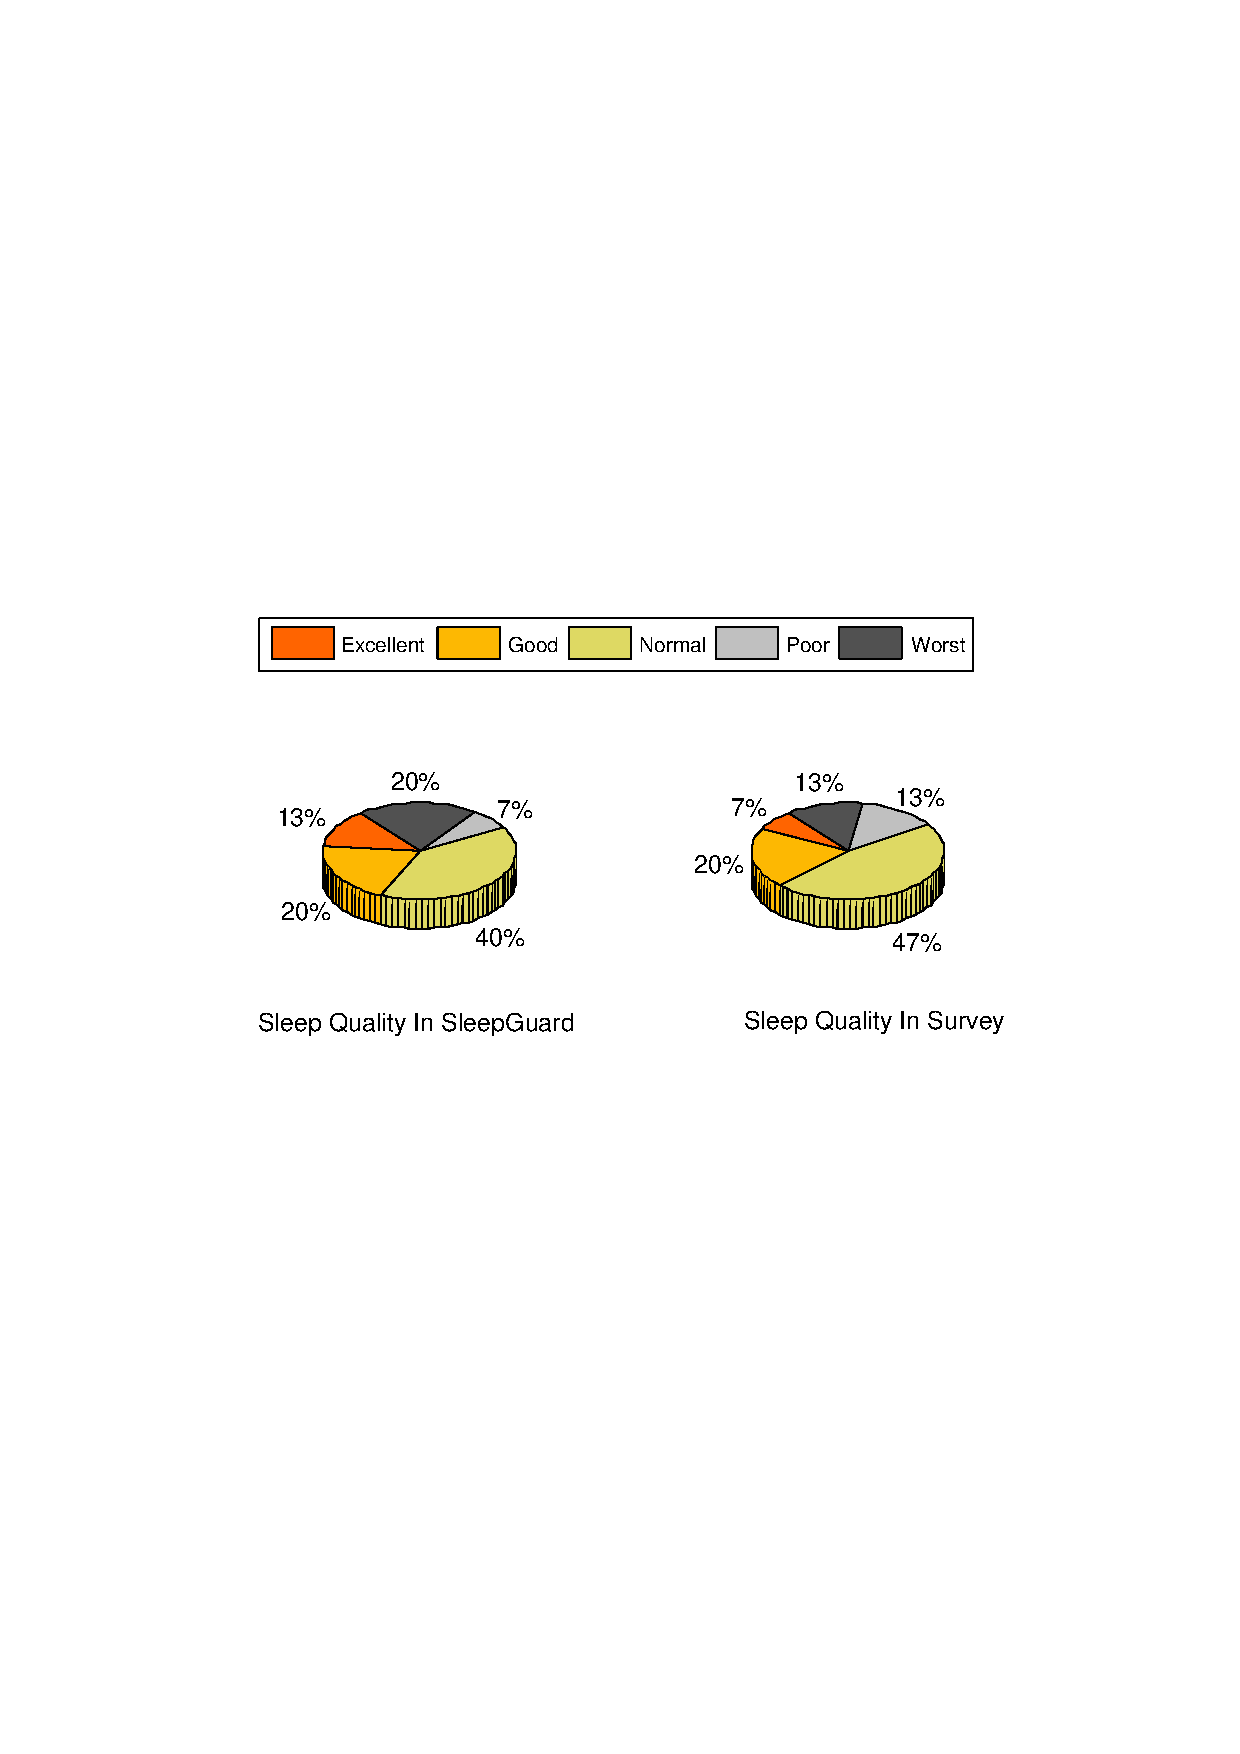
\includegraphics[width=0.52\linewidth]{Figures/quality.pdf}
 %\caption{Participants' sleep quality distribution}\label{fig:quality}
%\end{figure}
